\chapter{Architektura a návrh aplikace}
\label{sec:navrh}
Tato kapitola bude zaměřena na další fázi vyvýjeného nástroje a to na popis architektury a zvolených technologií, způsobu uložení dat a návrh uživatelského rohraní. U jednotlivých popisů bude uvedeno z jakých důvodu byly jednotlivé návrhové rozhodnutí učiněny. 

\section{Architektura systému}
Vzhledem k tomu, že byl jeden z hlavních požadavků na vyvýjený nástroj, umožnit přístup k aplikaci jedním či více uživateli zároveň, jevila se jako nejlepší možnost vytvořit webovou aplikaci dostupnou na zařízeních disponující webovým prohlížečem a připojením k internetu. Webové aplikace fungují na známé a rozšířené architektuře klient-server. Tato architektura dělí systém na klienta(uživatele) a server, kteří spolu komunikují, v případě webových aplikací, skrze internetový protokol HTTP. Zjednodušeně by se tato komunikace dala popsat jako série požadavků klienta a odpovědí ze strany serveru. 

Ještě před několika lety tento způsob tvořil základ webových stránek a aplikací. Tato komunikace sebou bohužel přínáší i jisté nevýhody v podobě delší odezvy webových aplikací, nutnosti obnovení zobrazené stránky apod. Jednotlivé události vyvolané uživatelem se musí řešit na straně serveru, ten vygeneruje odpověď ve formě html souboru, který si uživatel následně zobrazí v prohlížeči. Moderní způsob tvorby webových aplikací je minimalizace této komunikace a přenechání zpracování požadavků na straně zařízení klienta. To je z pravidla umožněno díky Javascriptu, což je skriptovací jazyk, jehož běhovým prostředím je právě webový prohlížeč. Javascript jako takový je jazyk, ve kterém se relativně dobře a rychle tvoří jednoduché skripty, nicméně pro větší a komplexnější projekty byly vytvořeny jeho nadstavby a rozšíření, které zjednodušují vývoj, efektivitu a správu daných aplikací. 

Jak je vidět na obrázku \ref{fig:architecture}, který znázorňuje diagram nasazení, tak bylo použito hned několik těchto rozšíření. Na tomto obrázku je kromě klienta a webového serveru ještě znázorněn server sloužící pro persistentní uložení dat(databáze). Zde je komunikace rodělena přímo na požadavky typu CRUD neboli všchny operace, které se provádějí se záznamy databáze a odpovědi ve specifickém formátu pro danou technologii. Nicméně se jedná stále o komunikaci pomocí protokolu HTTP stejně jako v případě klienta a webového serveru. Dále je zde také nastíněno rozdělení dnešních webových aplikací a to na front-end a back-end. Rovnou by bylo dobré říci, že i když je zde webový server a back-end znázorněn opticky větší, tak se podstatná část úloh zpracovává na straně front-endu. 

\begin{figure}[h]
\centering
	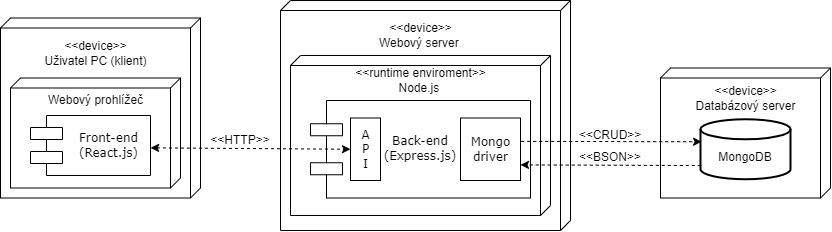
\includegraphics[width=1.0\textwidth]{Figures/deploymentDiagram.png}
	\caption{Diagram nasazení}
	\label{fig:architecture}
\end{figure}

\section{Použité technologie}
V této sekci boudou popsány technologie, které byly použit pro vývoj nástroje pro tvorbu FMEA. Jak bylo nastíněno v předchozí kapitole, tak byl zvolen přístup pro aplikaci, která zpracovává uživatelské požadavky převážně na straně klienta. Tyto aplikace se také nazývají SPA(Single Page Application). V praxi se pro tento typ vývoje používají především frameworky založené na Javascriptu. I z toho důvodu byl zvolen pro vývoj tzv. MERN stack, tedy použití technologií: MongoDB, Express, React, Node. 
\subsection{React}
Prvním rozšířením nebo též frameworkem je React, kterým je jedním z nejpoužívanějších frameworků pro vývoj webových aplikací na straně front-endu. Stejně jako ostatní populární javascriptové frameworky, jako například Angular nebo Vue, tak se aplikace dělí na jednotlivé bloky, které se nazývají komponenty. Komponenty spolu přinášejí obdobné výhody jako když hovoříme o třídách a objektech v objektově orientovaném programování. Zápisů komponent je více, ale obecně obsahují stav, vlastní programovou logiku v podobě metod a návratovou funkci ve formě html elementu.  

S tím také souvisí přístup, který se používá v Reactu a to je virtuální DOM. DOM je vlastně objektová reprezetace stromové struktury elementů, kterou obsahuje každý html kód. Tento strom se běžně používá pro manipulaci s elementy pomocí javascriptu. React přišel s nápadem, kdy interně pracuje s vlastní verzí této struktury a při změnách na základě události na stránce provádí aktualizace pouze ovlivněných komponent danou změnou. Určení se provádí na základě porovnání původních a aktualizovaných DOM objektů. Také závisí i na tom, jak programátor danou aplikaci dekomponuje. 

Dalším vlastností Reactu je možnost komibinace html kódu a programové logiky. To je skutečnost, která je řešena i v jiných frameworcích pro web. V Reactu se jedná o vlastní formát souboru s příponou .jsx, která umožňuje uvnitř html kódu komponent psát javascript pomocí kombinace symbolu '\$' a složených závorek. Nejčastěji se toto používá pro vložení hodnoty proměnných nebo například použití cyklu, který v každé iteraci vytváří nějakou sadu html elementů. 



\subsection{Node}
Node je běhovým prostředím pro Javascript na straně serveru postavený na Chrome V8 Javascript enginu. Javascript je navržen pro běh v prohlížeči a proto byl vytvořen Node, který umožňuje vytvářet aplikace na back-endu v tomto jazyku. Architektura Nodu je založena na tzv. smyčce událostí, kdy jsou postupně zachytávány uživatelské požadavky v rámci jednoho vlákna a dále přiděleny jednotlivým asynchroním vláknům. 

Další velice důležitou součástí Nodu je NPM(Node Package Manager), což je balíčkovací ekosystém, který umožňuje vývojáři přidávat balíčky(knihovny) do svého projektu pomocí konzole. Jedná se o jednu z největších databází knihoven na světě. V době psaní tohoto textu se počet odahaduje na více než 2.1 milionů balíčků. Díky tomuto faktu je vývoj webových stránek opravdu zjednodušen. V praxi se dá postupovat tak, že si vývojář navrhne strukturu své aplikace, vytvoří nějaké základní komponenty a pak prakticky pro jakoukoli funkcionalitu chce si může vybrat z nabídky několika balíčků, které jsou k dispozici. Vybraný balíček si pak jednoduše nainstaluje pomocí příkazu v konzole a pomocí dostupné dokumentaci pouze přidá požadavanou komponentu, metodu atd. Seznam všech balíčku obsahuje soubor s názvem package.json, který také vyjadřuje seznam závislostí.  

\subsection{Express}
Express je rychlý, nezávislý framework pro Node zjednodušující vývoj aplikací na back-endu. Idyž jsou snahy o to přesunout většinu zpracování na klienta, tak je stále potřeba komunikace se serverem například v případě prací se záznamy v databázi. Tato komunikace probíhá na základě HTTP protokolu a také pomocí základních metod, které se používají při tvorbě tzv. API, které slouží jako komunikační bod pro klienta. Nejčastěji používáné metody jsou GET, POST, PUT, DELETE. Express umožňuje psaní metod pro zpracování těchto požadavků. Metody obsahují v parametrech vždy atribut pro definici požadavku a odpověď, která slouží jako navratová hodnota.   

\subsection{MongoDB}
Pro persistentní uložení dat byla nakonec vybrána No-SQL databáze MongoDB spolu s Mongoose ODM. Důvod výběru Mongo databáze i krátký popis již byl zmíněn v kapitole \ref{sec:pozadavekMongo}, kde byl vysvětlen důvod zamítnutí systémového požadavku na tvorbu relační databáze. 

Mongoose je javascriptová knihovna, která vytváří propojení mezi MongoDB a běhovým prostředí Node. Označení ODM se používá pro databáze založené na ukládání dokumentů oproti klasickému ORM používaném v relačních databázích. Výhoda Mongoose je, že nabízí několik základních metod pro připojení k databázovému serveru, vytvoření schémat pro ukládání dokumentů a metod pro jejich manipulaci. 

\section{Návrh datové vrstvy}
Tato sekce se bude zabývat popisem a ukázkou toho, jak se v aplikaci pracuje s daty. Jak je možné vidět na obrázku \ref{fig:db} znázorňující relační vztahy čistě v rámci atributů analýzy, tak se jedná o relativně dosti provázanou strukturu. Zjednodušeně diagram obsahuje tabulku pro hlavičku analýzy, dále se následující tři kroky analýzy skládájí vždy ze tří úrovní, kdy spolu jednotlivé úrovně mezi sebou navzájem souvisí. Pátý a šestý krok analýzy je součástí třetí úrovně analýzy selhání, která je s ní pevně spjata. V návrhu je vidět, že mezi atributy převládají vazby 1-N a byly detailněji popsány již v teoretické části práce. Co se týká atributů objektů, tak prakticky každý objekt obsahuje atribut ID pro identifikaci a Name, který odpovídá hodnotě vyplněného pole hodnotícím týmem. Pro zajímvaost ještě možná dobré zmínit atribut Initial Severity(Vážnost), který se vyskytuje u selhání druhé úrovně narozdíl od ostatních hodnotících atributů. Je to z toho důvodu, že jedna hodnota tohoto atributu narozdíl od ostatních může odpovídat více objektům třetí úrovně. Nakonec se tento atribut vyskytuje i v rámci formuláře analýzy v odišném kroku analýzy narozdíl od atributů Výskyt a Detekce. Na závěr tohoto popisu je potřeba se krátce zmínit k dvěma typům analýzy: DFMEA a PFMEA. Oba dva tyto typy mají totožnou strukturu, co se týká počtu atributů, ale rozdílné názvy atributů hlavně v rámci analýzy struktury a funkcí a proto jsou v diagramu uvedeny obecně názvy objektů spolu s číslem označujícím úroveň. 

Návrh toho, jak ukládat data se ze začátku zdál docela jako komplikovanější úkol. Důvodem byl výběr knihovny, která slouží pro zobrazení stromové struktury v rámci grafického zobrazení analýzy. Pro práci s touto knihovnou je potřeba data udržovat v několikanásobně zanořeném objektu, který obsahuje atribut 'children'. Problém byl, jak vytvořit výše popsané relace v této datové struktuře Nakonec se toto podařilo pomocí toho, že v rámci objektu lze jeho atributy uložit jako pole dalších objektů, tím pádem šlo vytvořit tímto způsobem požadované vazby 1-N. Jedinou nevýhodou tohoto řešení bylo to, že některé záznamy musí být redundatní a operace aktualizace a mazání byly taktéž trochu složitější. Nicméně nespornou výhodou toho, že se podařilo spravovat všechna data v rámci jednoho zanořeného objektu bylo to, že se dala velice efektivně využít databáze založená na ukládání dat pomocí dokumentů. Pomocí tohoto způsobu uložení dat, lze rovnou uložit celý objekt bez jakékoli nutnosti transformace dat např. pomocí návrhového vzoru DTO, který slouží právě pro podobné situace. 

\begin{figure}[H]
\centering
	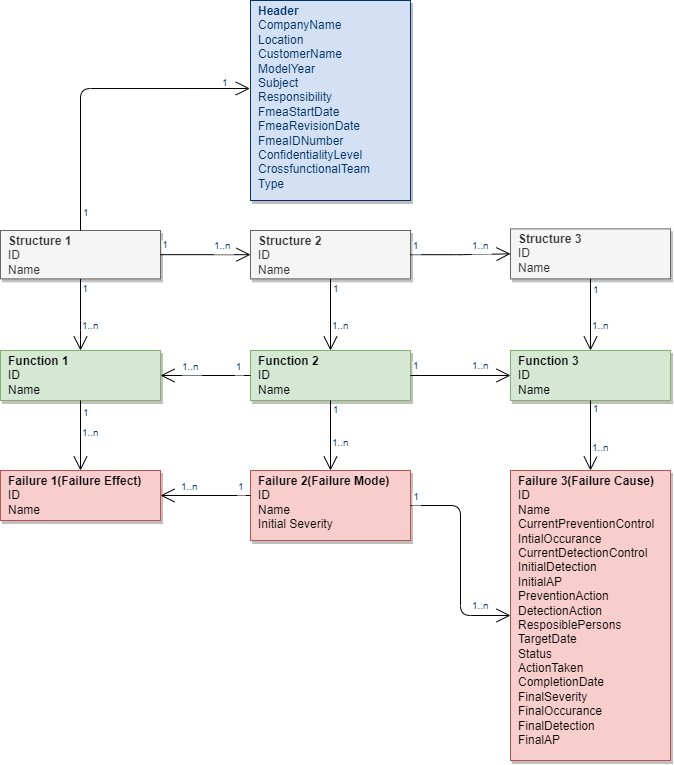
\includegraphics[width=1.0\textwidth]{Figures/db_model.png}
	\caption{Konceptuální diagram }
	\label{fig:db}
\end{figure}

\section{Návrh uživatelského rozhraní}
Poslední část této kapitoly bude zaměřena na Návrh uživatelského rozhraní. Jak bylo řečeno v úvodu kapitoly, tak bude snaha vyvynout tzv. Single Page Application. A to nejen z pohledu zpracování požadavků, ale také shodou okolností z pohledu uživatelského rohraní. Vize je taková, že bude existovat jedna stránka obsahující grafický i textový pohled na analýzu. Úpravy atributů a ostatní funkce budou vyřešeny v rámci modálních oken. Uživatel tak bude mít všechny funkce na jedné stránce bez nutnosti přecházet na jiné odkazy v rámci webu. 

Důležitým rozhodnutím při návrhu uživatelského rozhraní bylo jaký zvolit formát tabulky. Možností existuje více, ale v základu se běžně používá řešení, kdy jsou všechny kroky tabulky za sebou v řádku. Problém v tomto zobrazení je ten, že se velice obtížně zobrazují všechny relace v jednom řádku při současném slučování buněk. Zároveň jednotlivé atributy mezi sebou v rámci kroků analýzy souvisí, což v nemusí být v řádku bez barevného označení také hned zřejmé. Proto bylo nakonec zvoleno jedno z novějších zobrazení, které se vyskytuje například v posledním vydání přiručky FMEA pro automotive.[..] V rámci tohoto zobrazení jsou první tři kroky analýzy nad sebou, což výrazně zvyšuje čitelnost souvisejích prvků. Zbytek kroků vycházející z odhalených přičin selhání je již pak bez problému zobrazen v řádku. Náhled tohoto formátu zobrazení lze vidět na obrázku \ref{fig:ui}.

\begin{figure}[h]
\centering
	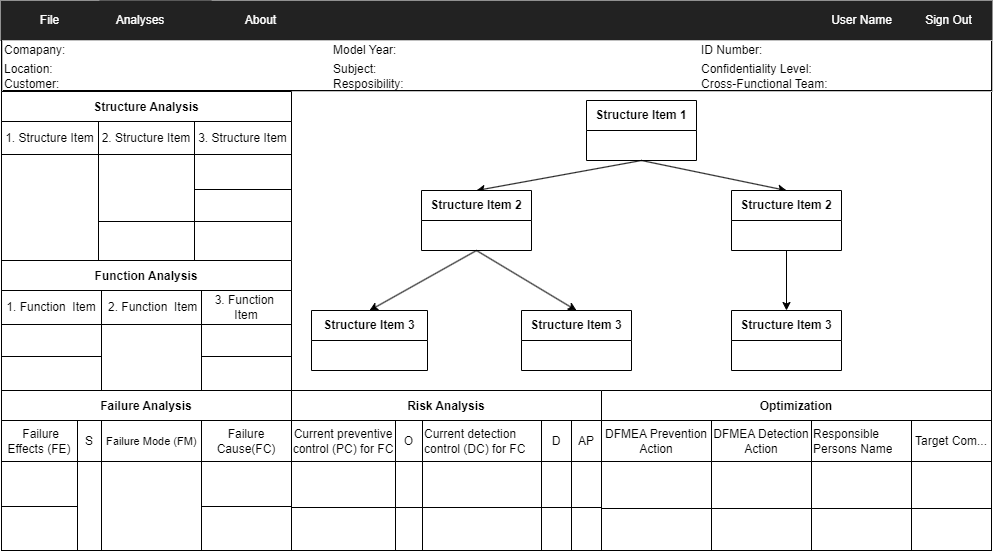
\includegraphics[width=1.0\textwidth]{Figures/mockup3.png}
	\caption{Návrh UI }
	\label{fig:ui}
\end{figure}